\section{Equivalência de Recursos}

	Para que um recurso R1 seja equivalente a um recurso R2, os serviços de R2 deverão estar presentes no conjunto de serviços de R1, mas R1 poderá ter outros serviços que não estão presentes em R2. Seja S(X), o conjunto de serviços do recurso X, então teríamos que $S(R1) \cap S(R2) = S(R2)$. 
	A figura~\ref{fig:equivalenciaDeRecursos} mostra esse relacionamento.
	Logo temos uma relação unidirecional de equivalência, visto que R2 não é equivalente a R1, pois não possui o serviço S3. Para dizer que um um recurso R1 é equivalente a um recurso R2, utilizaremos a seguinte notação: $R1 \implies R2$.
	
	\begin{figure}[ht]
		\center
		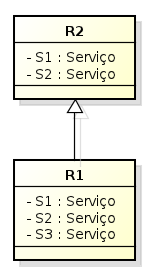
\includegraphics[scale=0.6]{imagens/equivalenciaDeRecursos}
		\caption{Exemplo de recursos equivalentes.}
		\label{fig:equivalenciaDeRecursos}
	\end{figure}

	Suponha uma situação em que $A \implies B$, $B \implies C$ e $C \implies A$, logo teríamos que $A \implies C$, o que seria uma relação circular, o que não faz sentido, pois concluiríamos que todos os recursos são iguais e não equivalentes. Devemos, portanto, garantir que não ocorra essa equivalência circular. Caso algum dispositivo queira registrar um novo \emph{driver} que cause essa inconsistência, devemos impedir e alertá-lo da ocorrência dessa inconsistência. 

\subsection{Consistência de Interface}

	A figura~\ref{fig:consistenciaInterface} mostra que o recurso R1 é equivalente ao recurso R3, mas embora possua um serviço de mesmo nome que o recurso R2,  seus parâmetros são diferentes, logo, não pode ser um mesmo serviço e os recursos não serão equivalentes..
	
	Para garantir que os recursos são equivalentes, devemos realizar três validações nas interfaces de cada serviço dos recursos:
	\begin{enumerate}
		\item Recurso:
			
			Os serviços devem pertencer ao mesmo recurso cujas classes padrões foram definidas anteriormente.
		
		\item Identificador do Serviço:

			Os serviços devem possuir os mesmos identificadores.

		\item Parâmetros:

			Os serviços devem possuir os mesmos parâmetros.
	\end{enumerate}

	Parte-se do princípio que não existirá interesse em camuflar um serviço malicioso ao expor uma interface compatível com a equivalência.

\begin{figure}[ht]
	\center
	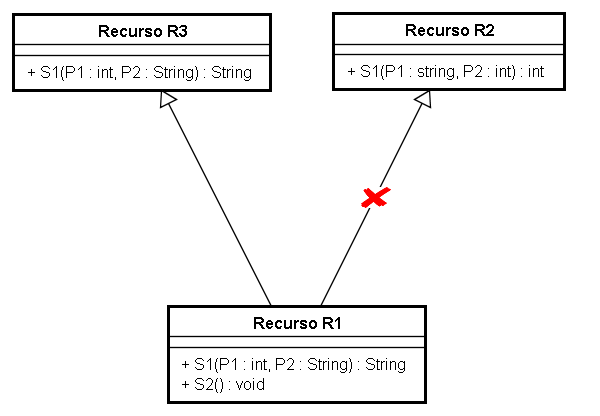
\includegraphics[scale=0.8]{imagens/consistenciaInterface}
	\caption{Exemplo de inconsistência de interface.}
	\label{fig:consistenciaInterface}
\end{figure}

\begin{comment}
----------------------------------------- REVER ----------------------------------------- \\
Desta forma, faz-se necessária uma maneira de classificar tais recursos imersos nos mais variados dispositivos presentes no \emph{smart space} e regidos pelo \emph{middleware}. Essa classificação facilitará o desenvolvimento de novos \emph{drivers} para futuras aplicações, pois tornará possivel a definição de interfaces pré-estabelecidas que representem classes de recursos. Outra vantagem decorrente é a possibilidade de seleção de recursos equivalentes, caso o provedor originalmente selecionado esteja indisponível. \\
----------------------------------------- REVER -----------------------------------------

COLOQUEI NO COMEÇO DA PROPOSTA
\end{comment}
